\begin{frame}\frametitle{Neutrino Oscillations Discovery}
%\scriptsize
%History of the neutrino oscillations discovery is described in the Griffiths textbook \cite{ref_Griffiths}, chapter 11.
%\begin{itemize}
%  \scriptsize
%  \item Homestake experiment, 1968
%  \tiny
%  \begin{itemize}
%     \item Chlorino radiochemical detector ($\nu_e + ^{37}Cl \rightarrow ^{37}Ar+e$) 
%     \item Sensitive to $\nu_e$ only 
%     \item Recorded $1/3$ of theoretically predicted neutrino flux
%     \item Solar neutrino problem postulated
%  \end{itemize}
%  \scriptsize
%  \item Bruno Pontecorvo proposes theory: neutrino can change flavor and thus $\nu_e$ converted to $\nu_\mu$ and/or $\nu_\tau$ and weren't registered. But at first it was believed the Homestake experiment made mistake
%  \item more neutrino experiments report lack of Sun electron neutrinos
%  \item Super-Kamiokande experiment, 1998 
%  \tiny
%  \begin{itemize}
%     \item Water Cherenkov detector ($\nu + e \rightarrow \nu + e$). 
%     \item Sensitive to all $\nu$ but detection efficency of $\nu_e$ is 6.5 times bigger
%     \item Recorded $45\%$ of theoretically predicted neutrino flux (assumed all $\nu$=$\nu_e$)
%  \end{itemize}
%  \scriptsize
%  \item Solar neutrino observatory (SNO), 2002
%  \tiny
%  \begin{itemize}
%     \item Heavy water Cherenkov detector ($\nu_e + d \rightarrow p+p+e$, $\nu+d \rightarrow n+p+\nu$, $\nu+e \rightarrow \nu+e$)
%     \item Sensitive to all $\nu$ but can separate $\nu_e$
%     \item Reported $\nu_e$ flux to be $35\%$ of the predicted flux
%  \end{itemize}
%  \scriptsize
%  \item Combining Super-Kamiokande and SNO results
%  \tiny
%  \begin{itemize}
%     \item $45\%=35\%+10\%$, $10\% \cdot 6.5 = 65\%$, $35\%+60\%=100\%$
%     \item Neutrino oscillations theory confirmed
%     \item Solar neutrino problem resolved
%  \end{itemize}
% $\nu_e + d \rightarrow p+p+e$, $\nu+d \rightarrow n+p+\nu$, $\nu+e \rightarrow \nu+e$
%\end{itemize} 
\end{frame}

\begin{frame}\frametitle{Theory. Two Neutrinos Case}
  \scriptsize
  \begin{center}
  $\nu_1=\nu_{\mu}cos\theta-\nu_esin\theta$\\
  $\nu_2=\nu_{\mu}sin\theta+\nu_ecos\theta$\\
  \end{center}
  \begin{center}
  $\nu_1(t)=\nu_1(0)e^{\frac{-iE_1t}{\hbar}}$, $\nu_2(t)=\nu_2(0)e^{\frac{-iE_2t}{\hbar}}$ $\leftarrow$ from quantum mechanics\\
  \end{center}
  Suppose, at t=0 there were $\nu_e(0)=1$, $\nu_\mu(0)=0$\\
  Then: $\nu_1(0)=-sin\theta$, $\nu_2(0)=cos\theta$, $\nu_1(t)=-{sin\theta}e^{\frac{-iE_1t}{\hbar}}$, $\nu_2(t)=-{cos\theta}e^{\frac{-iE_2t}{\hbar}}$\\
  Therefore, we are getting the system:\\
  \begin{center}
  $-{sin\theta}e^{-{{iE_1t} \over \hbar}}=\nu_\mu(t)cos\theta-\nu_e(t)sin\theta$,\\
  $-{sin\theta}e^{-{{iE_2t} \over \hbar}}=\nu_\mu(t)sin\theta-\nu_e(t)cos\theta$\\
  \end{center}
  By solving this sytem for $\nu_e$ and $\nu_\mu$, one would get:\\
  \begin{center}
  $P_{\nu_e \rightarrow \nu_\mu}=|\nu_\mu(t)|^2=[{sin2\theta}sin{\frac{(E_1-E_2)t}{2\hbar}}]^2$,\\
  $P_{\nu_e \rightarrow \nu_e}=|\nu_e(t)|^2=1-[{sin2\theta}sin{\frac{(E_1-E_2)t}{2\hbar}}]^2$\\
  \end{center}
\end{frame}

\begin{frame}\frametitle{Theory. Two Neutrinos Case}
  \begin{center}
  $P_{\nu_e \rightarrow \nu_\mu}=|\nu_\mu(t)|^2=[{sin2\theta}sin{\frac{(E_1-E_2)t}{2\hbar}}]^2$,\\
  $P_{\nu_e \rightarrow \nu_e}=|\nu_e(t)|^2=1-[{sin2\theta}sin{\frac{(E_1-E_2)t}{2\hbar}}]^2$\\
  \end{center}
  Therefore, for freely travelling neutrinos, if $\nu_e$ was emmitted, at any point there is a certain probability to register $\nu_e$ or $\nu_\mu$ and those probablities change with time periodically, by $~[sin(At)]^2$ law. That's why the phenomenon is called the neutrino oscillations.
  Suppose momenta $p_1=p_2$. Then using $E^2=p^2+m^2$ and assuming $m_{1,2}<<E_{1,2}$, the probablities will take forms of\\
  \begin{center}
  $P_{\nu_e \rightarrow \nu_\mu}=|\nu_\mu(t)|^2=[{sin2\theta}sin{\frac{(E_1-E_2)t}{2\hbar}}]^2=[{sin2\theta}sin{\frac{(m_1^2-m_2^2)c^3}{4\hbar{E}}z}]^2$\\  
  \end{center}
\end{frame}

\begin{frame}\frametitle{Theory. Three Neutrinos Case}
  \scriptsize
  Oscillations are determined by Pontecorvo-Maki-Nakagava-Sakata (PMNS) matrix:\\
  \begin{center}
  $ \begin{pmatrix} \nu_{e} \\ \nu_{\mu} \\ \nu_{\tau} \\ \end{pmatrix}
  = U_{PMNS}\cdot \begin{pmatrix} \nu_{1} \\ \nu_{2} \\ \nu_{3} \\ \end{pmatrix} = 
  \begin{pmatrix}
  U_{e1} & U_{e2} & U_{e3} \\
  U_{\mu1} & U_{\mu2} & U_{\mu3} \\
  U_{\tau1} & U_{\tau2} & U_{\tau3} \\
  \end{pmatrix}
  \cdot
  \begin{pmatrix} \nu_{1} \\ \nu_{2} \\ \nu_{3} \\ \end{pmatrix}$\\
  \end{center}
  The $U_{PMNS}$ matrix depends on three neutrino mixing angles ($\theta_{12}$, $\theta_{23}$, $\theta_{13}$) and CP-violating phase $\delta_{CP}$. If define $c_{ab}=cos\theta_(ab)$, $s_{ab}=sin\theta_(ab)$, the $U_{PMNS}$ matrix can be splitted into three multipliers, each would be responsible for mixing of one pair of neutrino flavors:\\
  \begin{center}
  $U_{PMNS} =
  \begin{pmatrix}
  1 & 0 & 0 \\
  0 & c_{23} & s_{23} \\
  0 & -s_{23} & c_{23} \\
  \end{pmatrix}
  \cdot
  \begin{pmatrix}
  c_{13} & 0 & e^{i\delta_{CP}}s_{13} \\
  0 & 1 & 0 \\
  -e^{i\delta_{CP}}s_{13} & 0 & c_{13} \\
  \end{pmatrix}
  \cdot
  \begin{pmatrix}
  c_{12} & s_{12} & 0 \\
  -s_{12} & c_{12} & 0 \\
  0 & 0 & 1 \\
  \end{pmatrix}$ \\
  \end{center}
\end{frame} 

\begin{frame}\frametitle{Theory. Three Neutrinos Case}
  \scriptsize
  The probability amplitudes of neutrino mixing are defined by parameters of the $U_{PMNS}$ but, analogous to simplified two-neutrino case described above, the differences of squares of neutrino masses also contribute to the probability. There are two independent expressionce for squares of masses differences: ${\Delta}m_{12}^2 = m_1^2-m_2^2$ and ${\Delta}m_{32}^2 = m_3^2-m_2^2$. Mass differences were measured in other neutrino oscillation experiments but the ${\Delta}m_{12}^2$ and ${\Delta}m_{32}^2$ present in the equations evenly and therefore the signs of these expressions were not measured. If the masses order as $m_3 > m_2 > m_1$, it's called normal neutrino mass hierarchy because other fundamental particles orders in a way that later generation particles have higher masses than lower generation particles. If the masses order as $m_1 > m_2 > m_3$ it's called inverted neutrino mass hierarchy. The mixing angles $\theta_{12}$, $\theta_{23}$, $\theta_{13}$ and differences of squared masses $|{\Delta}m_{12}^2|$ and $|{\Delta}m_{32}^2|$ are measured and give $U_{PMNS}$ matrix form of\\
  \begin{center}
  $|U_{PMNS}| \sim
  \begin{pmatrix}
  0.8 & 0.5 & 0.2 \\ 0.5 & 0.6 & 0.6 \\ 0.2 & 0.6 & 0.8 \\
  \end{pmatrix}$\\
  \end{center}
  The CP-violating phase $\delta_{CP}$ is unknown.\\*
  The analogous matrix for quark mixing, Cabibbo-Kobayashi-Maskawa (CKM) matrix $V_{CKM}$, is much more diagonal:\\*
  \begin{center}
  $|V_{CKM}| \sim
  \begin{pmatrix}
  1 & 0.2 & 0.004 \\ 0.2 & 1 & 0.04 \\ 0.008 & 0.04 & 1 \\
  \end{pmatrix}$\\
  \end{center}
  One of the important questions in modern particle physics is why the quark mixing angles are so much smaller than neutrino mixing angles and the other important question is whether there is any relationship between quark and neutrino mixing matrices.\\
\end{frame}

\begin{frame}\frametitle{$P(\nu_\mu \rightarrow \nu_e)$ at a baseline of 1300 km}
  \scriptsize
  \begin{figure}
  \label{fig:LBNF_oscProbability}
  \centering
  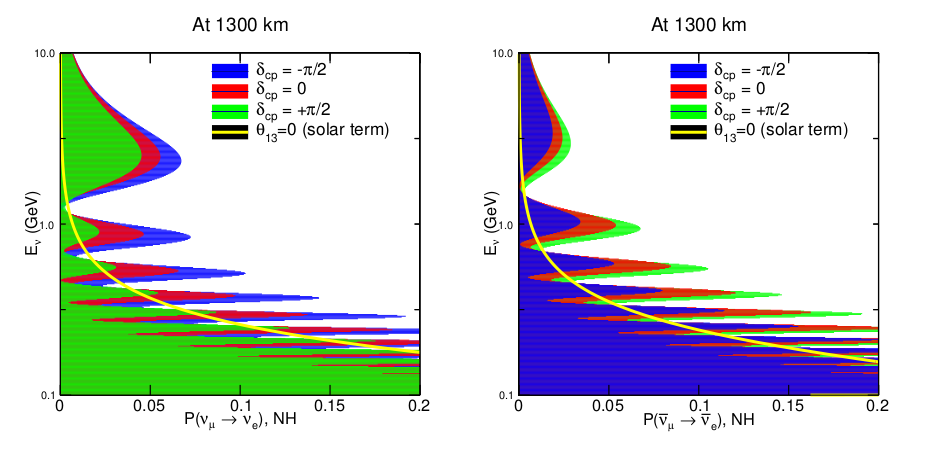
\includegraphics[width=0.98\textwidth, keepaspectratio=true]{figs/LBNF_oscProbability.png}
  \\$P(\nu_\mu \rightarrow \nu_e)$ at a baseline of 1300 km, as a function of neutrino energy. Left - neutrinos, right - antineutrinos. Figure is taken from the LBNF CDR draft, volume physics\cite{ref_LBNFdoc_volume-physics}
  \end{figure}
\end{frame}

\begin{frame}\frametitle{Available Experimental Results \cite{ref_PDG}}
  \scriptsize
  \begin{itemize}
    \item $sin^2(2\theta_{12})$=$0.846\pm0.021$
    \item $sin^2(2\theta_{23})$=$0.999^{+0.001}_{-0.018}$
    \item $sin^2(2\theta_{23})$=$1.000^{+0.000}_{-0.017}$
    \item ${\Delta}m^2_{21}$=$(7.53\pm0.18) \cdot 10^{-5} eV^2$
    \item ${\Delta}m^2_{32}$=$(2.44\pm0.06) \cdot 10^{-3} eV^2$ $\leftarrow$ if $m_3>m_2>m_1$
    \item ${\Delta}m^2_{32}$=$(2.52\pm0.07) \cdot 10^{-3} eV^2$ $\leftarrow$ if $m_1>m_2>m_3$
    \item CP-violation phase $\delta_{CP}$ - not measured
    \item mass hierarchy - not determined
  \end{itemize} 
\end{frame}
